\chapter{The CMS Experiment at the LHC}\label{ch:exp}
This measurement was performed using data collected by the CMS Experiment, one of the multipurpose detector experiments at the LHC. This chapter details the technical design and operation of the LHC and CMS. 

%%%%%%%%%%%%%%%%%%%%%%%%%%%%%%%%%%%%%%%%%%%%%%
%            LHC 
%%%%%%%%%%%%%%%%%%%%%%%%%%%%%%%%%%%%%%%%%%%%%%

\section{The Large Hadron Collider}
The Large Hadron Collider is an 26.7 km-circumference accelerator designed to circulate protons or heavy nuclei in opposing directions to facilitate the study of fundamental physical interactions. It is housed in an underground tunnel, crossing the French-Swiss border, at a depth between 40m to 170m. This tunnel was previously home to the electron-positron collider, LEP. The LHC and accelerator complex at CERN are shown in Figure~\ref{fig:cern_accel_cartoon}.

%insert figure. 
% add figure
\begin{figure}
\centering
  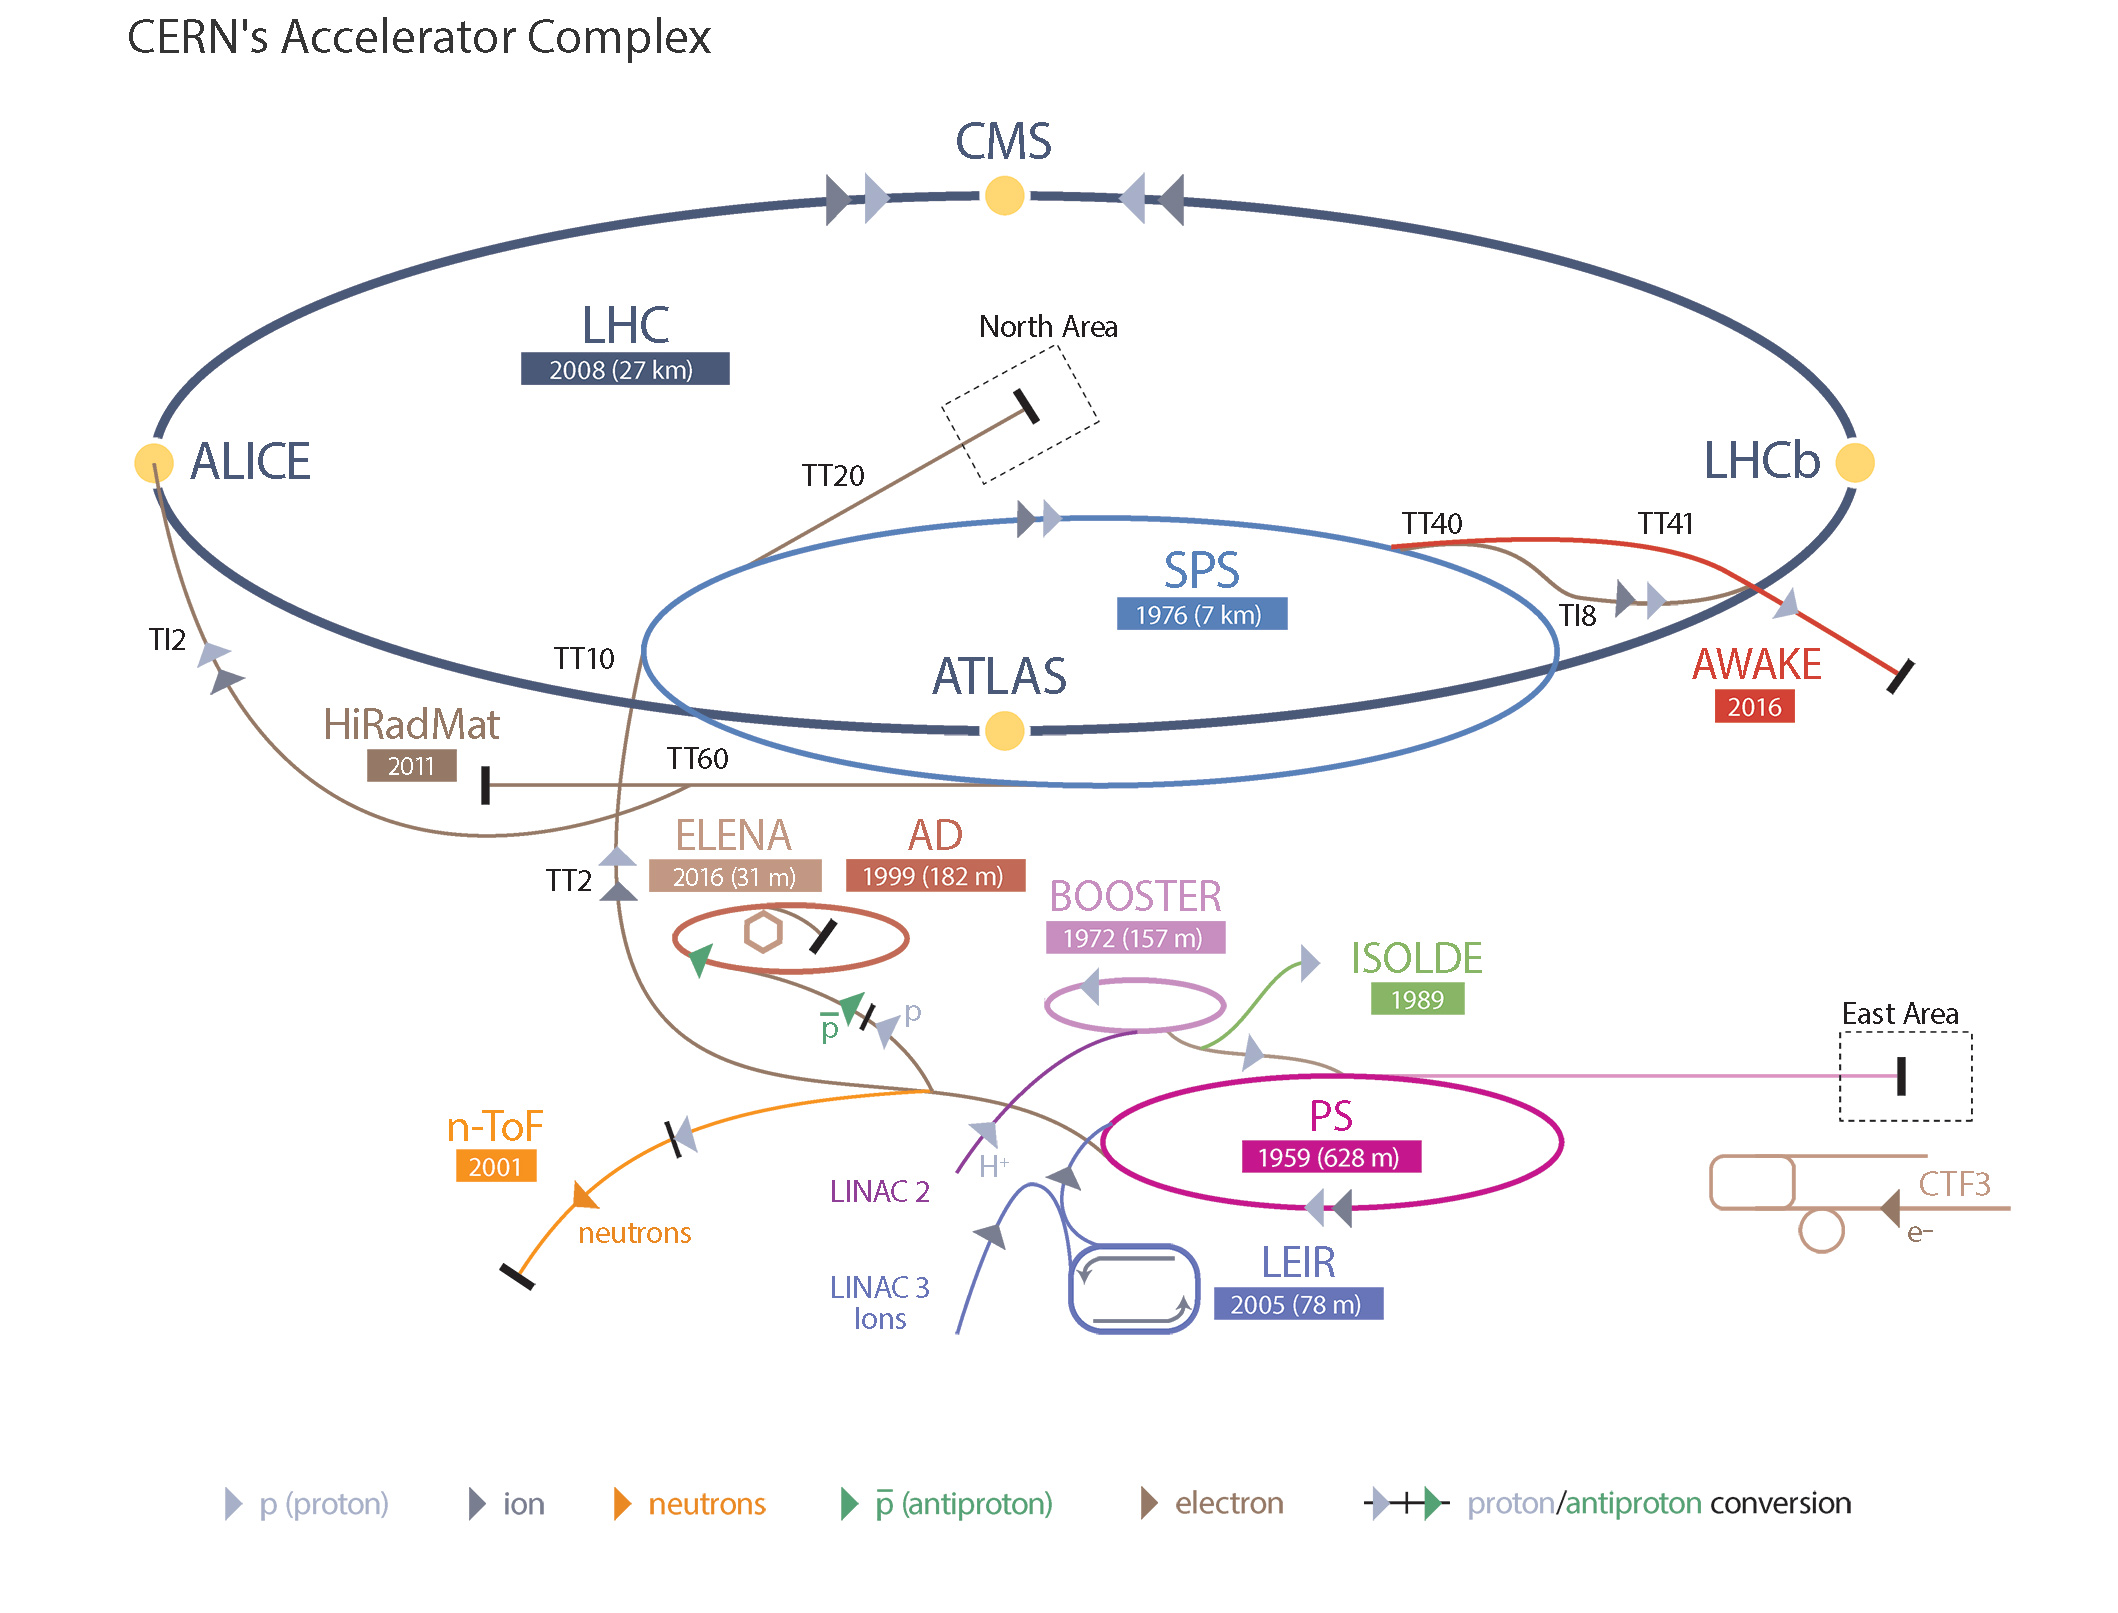
\includegraphics[width=0.75\linewidth]{plots/LHC/CERN_accelerators.jpg} %% put in this figure
  %https://cds.cern.ch/record/40524
  \caption{Illustration of the full accelerator complex at CERN, including the pre-accelerators, the LHC, and the major collision halls at the LHC.  \protect\cite{LHC_Accel_Cartoon}}
  \label{fig:cern_accel_cartoon}
\end{figure}

%%%%%%%% Producing Protons & pre-accelerator 
\subsubsection{LHC Pre-Accelerators}
Protons are produced by ionizing hydrogen gas, which are accelerated to 50 \MeV by LINAC2, and injected into the Proton Synchroton Booster. The PSB then brings the protons to 1.6 \GeV for injection into the Proton Synchrotron (PS). The PS takes six proton bunches, splits each into three prior to acceleration to 25 \GeV, then subsequently splits each bunch into four prior to injection into the Super Proton Synchroton (SPS), resulting in 72 bunches injected into the SPS. The SPS can receive up to 4 sets of 72 bunches from the PS, accelerating them to 450 \GeV per proton for injection into the LHC where they are further accelerated to a maximum of 6.5 \TeV per proton. Bunches from SPS can be injected into the LHC up to 24 times, for a minimum spacing of 25 \ns between bunch crossings\cite{Benedikt:2004wm}. 

\subsubsection{The Large Hadron Collider}
After injection into the LHC, protons are accelerated by radio-frequency (RF) cavities to an energy of 6.5 \TeV. 
The trajectory of the protons around the ring is controlled by 1232 niobium-titanium wire superconducting dipole magnets, 15m in length, which are cooled by liquid Helium to a temperature of 1.9 K and have a magnetic field strength of 8.33 T. These dipole magnets are responsible for bending the proton beams in the appropriate direction around the LHC. Superconducting quadrupole magnets, 5-7 m in length, are used to focus the proton bunches.  The focusing quadrupoles are located near the collision points, to produce a more focused beam in preparation for collisions. Higher-order multipole magnets are also used for beam focusing and control. 
The beams circulated in the LHC are proton-proton, so the same beampipe cannot be used for both beams. Therefore a twin-bore magnet design is employed, where both beampipes are situated on the interior of the same magnet. A cross section of an LHC dipole is shown in Figure \ref{fig:lhc_dipole} \cite{Bruning:2004ej}.
% add figure
\begin{figure}
\centering
  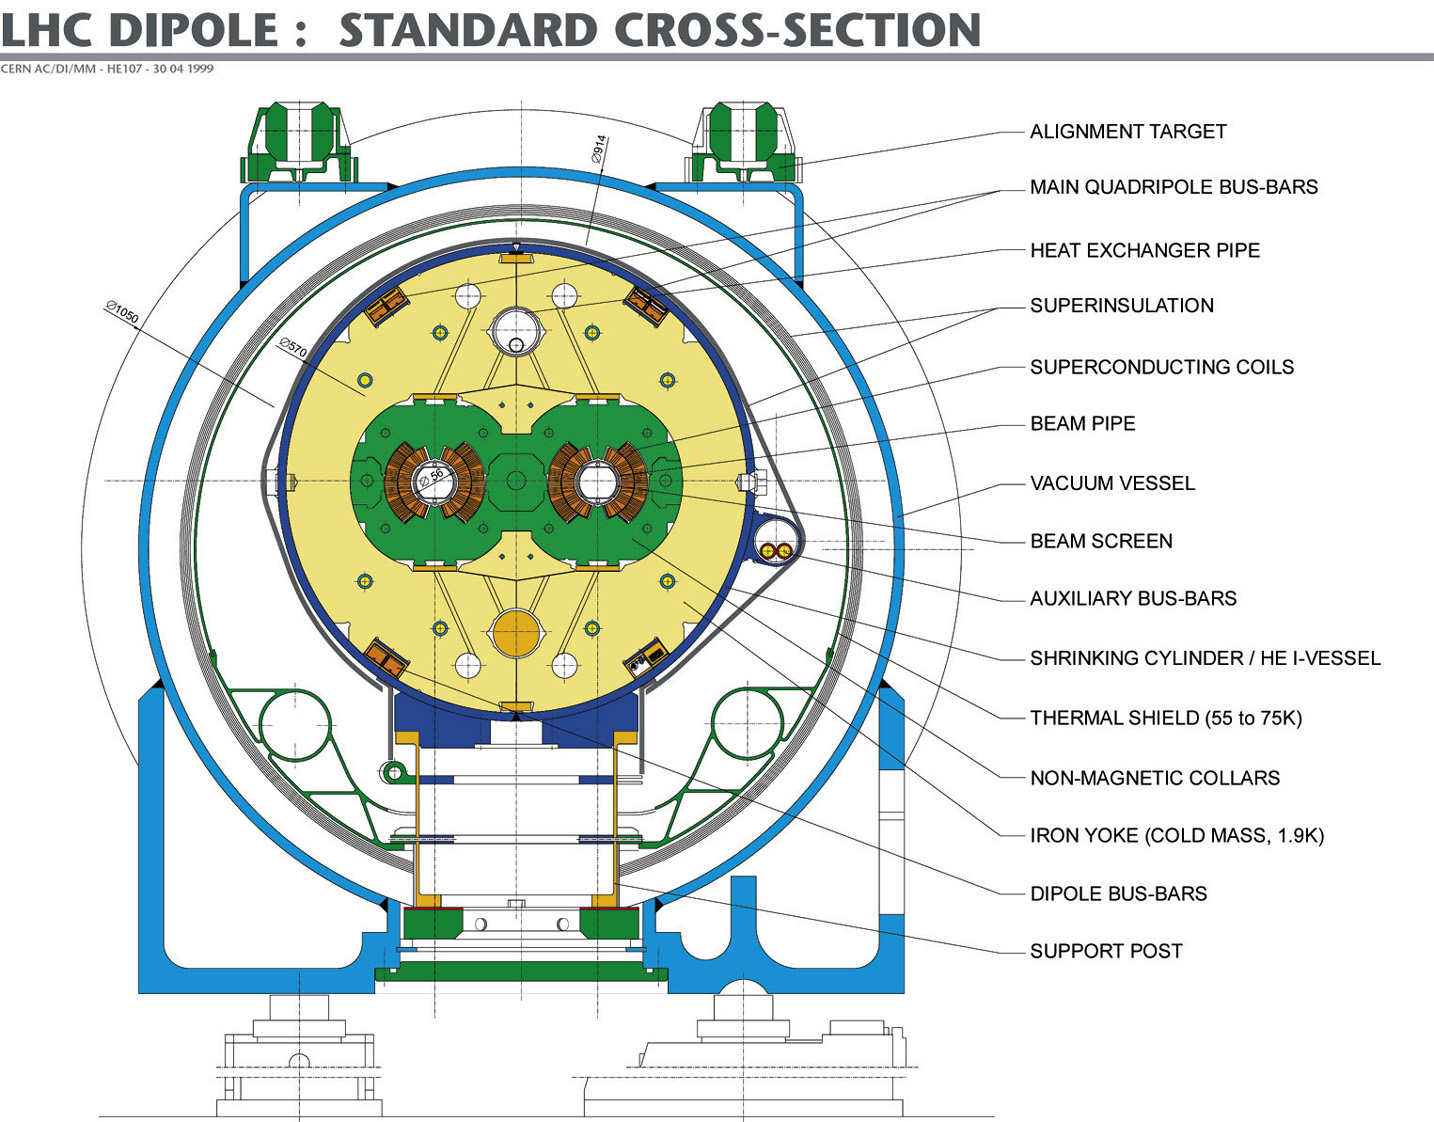
\includegraphics[width=0.5\linewidth]{plots/LHC/LHC_dipole.jpeg} %% put in this figure
  %https://cds.cern.ch/record/40524
  \caption{Cross-section of an LHC dipole magnet, showing the twin-bore design to accomodate the beampipes. \protect\cite{Team:40524}}
  \label{fig:lhc_dipole}
\end{figure}

Collisions occur where the beams intersect each other, located at multiple points around the LHC: Point 1 (ATLAS), Point 2 (ALICE), Point 5 (CMS), and Point 8 (LHCb). 